\documentclass[12pt,english]{article}
\usepackage{mathptmx}

\usepackage{color}
\usepackage[dvipsnames]{xcolor}
\definecolor{darkblue}{RGB}{0.,0.,139.}

\usepackage[top=1in, bottom=1in, left=1in, right=1in]{geometry}

\usepackage{amsmath}
\usepackage{amstext}
\usepackage{amssymb}
\usepackage{setspace}

\usepackage[authoryear]{natbib}
\usepackage{url}
\usepackage{booktabs}
\usepackage[flushleft]{threeparttable}
\usepackage{graphicx}
\usepackage[english]{babel}
\usepackage{pdflscape}
\usepackage[unicode=true,pdfusetitle,
 bookmarks=true,bookmarksnumbered=false,bookmarksopen=false,
 breaklinks=true,pdfborder={0 0 0},backref=false,
 colorlinks,citecolor=black,filecolor=black,
 linkcolor=black,urlcolor=black]
 {hyperref}
\usepackage[all]{hypcap}
\usepackage{breakurl}

\linespread{2}

\begin{document}

\begin{singlespace}
\title{Human Capital Disclosure and Earnings Response Coefficients:
       Evidence from SEC Regulation S-K}
\end{singlespace}

\author{Yeyang Zhou\thanks{University of Oklahoma.\
E-mail~address:~\href{mailto:yeyangzhou@ou.edu}{yeyangzhou@ou.edu}}}

\date{April 27, 2026}

\maketitle

\begin{abstract}
\begin{singlespace}
This paper examines whether the SEC Regulation S-K human capital disclosure
(HCD) mandate, effective November 2020, increased the informativeness of
earnings announcements for investors, and whether this effect is stronger for
firms that voluntarily disclosed more human capital information before the
mandate. Using a cross-sectional difference-in-differences design centered on
firm-level pre-mandate HCD intensity measured via the \citet{demers2024}
lexicon, I find that firms with greater pre-period HCD intensity experience a
larger post-mandate increase in earnings response coefficients (ERC). The
triple-interaction estimate $\hat{\beta}_4$ is positive and statistically
significant across multiple return windows and UE specifications, and is robust
to excluding the confounding FY2020 COVID-19 shock. These results are
consistent with the mandate formalizing and credibilizing existing human
capital signals, thereby improving the precision with which investors map
earnings news to future cash flows.
\end{singlespace}
\end{abstract}

\vfill{}
\pagebreak{}


%================================================
\section{Introduction}\label{sec:intro}
%================================================

\begin{itemize}
    \item The SEC amended Regulation S-K Item~101(c) in November 2020,
          replacing the prior checklist-based requirement (disclose employee
          headcount) with a principles-based mandate to describe human capital
          resources, including material measures related to attraction,
          development, and retention of employees.
    \item Because the SEC did not prescribe specific metrics, firms vary
          substantially in how much human capital information they include in
          their 10-K filings both before and after the mandate.
    \item Research question: Do firms with greater pre-mandate HCD intensity
          experience a larger increase in ERC following the mandate?
    \item Two competing mechanisms:
          \begin{itemize}
              \item \emph{Information shock channel}: Low-HCD firms face a
                    larger information shock as the mandate forces previously
                    private information into public filings, which could raise
                    their ERC more.
              \item \emph{Credibility/formalization channel}: High-HCD firms
                    benefit more because the mandate formalizes and validates
                    their existing signals under legal liability, improving
                    signal credibility and investor confidence.
          \end{itemize}
    \item Identification challenge: The mandate coincides with the COVID-19
          crisis (peak: FY2020). A simple pre/post comparison cannot separate
          regulation from crisis effects. This paper addresses this by using
          cross-sectional variation in pre-period HCD intensity as treatment
          exposure, which is predetermined with respect to both the mandate
          and COVID-19.
    \item Main finding: $\hat{\beta}_4 > 0$ and significant, consistent with
          the credibility/formalization channel. High-HCD firms see a
          differentially larger ERC increase post-mandate. The result is
          robust to excluding FY2020 and to multiple return and UE
          specifications.
    \item Contribution: First paper to examine ERC consequences of the 2020
          HCD mandate using a cross-sectional identification strategy that
          cleanly separates the mandate from COVID-19.
\end{itemize}


%================================================
\section{Literature Review}\label{sec:litreview}
%================================================

The literature on earnings response coefficients dates to \citet{ball1968},
who first documented that accounting earnings convey information reflected in
stock prices. \citet{collins1989} extended this framework to show that ERC
varies cross-sectionally with firm characteristics that proxy for the quality
of the information environment, including firm size, growth, and risk.

\citet{verrecchia2001} provides the theoretical foundation for the
disclosure--ERC link: voluntary disclosure reduces information asymmetry
between managers and investors, lowering the cost of capital and improving
price efficiency. \citet{lambert2007} formalize this mechanism, showing that
higher-quality accounting information reduces investors' estimation risk and
therefore strengthens the market's response to earnings news.

\begin{itemize}
    \item Human capital disclosure literature: Prior work documents that firms
          vary widely in the quantity and quality of voluntary HCD in annual
          reports \citep{demers2024}.
    \item Closest prior paper: \citet{skinner2026} show that integrated HCD
          helps investors process financial news, providing direct evidence
          that human capital information affects earnings informativeness.
    \item This paper differs by (i) exploiting the 2020 regulatory shock as a
          quasi-natural experiment, (ii) using a cross-sectional
          difference-in-differences design to address COVID-19 confounding,
          and (iii) directly estimating the differential ERC change for
          high-vs-low HCD firms.
\end{itemize}


%================================================
\section{Data}\label{sec:data}
%================================================

\begin{itemize}
    \item \textbf{Financial data}: Annual firm fundamentals from Compustat
          \texttt{funda} (Wharton Research Data Services, WRDS). Standard
          filters applied: \texttt{INDL/STD/D/C}, one observation per
          firm-year. Sample: all fiscal years with non-missing earnings and
          market value.
    \item \textbf{Stock returns}: Monthly returns from CRSP \texttt{msf\_v2};
          market returns from \texttt{msi}. Filters: common equity
          (\texttt{ShareType=NS}), domestic (\texttt{USIncFlg=Y}), listed on
          NYSE/AMEX/NASDAQ. Linked to Compustat via CCM
          (\texttt{ccmxpf\_lnkhist}), link types LU/LC, primary links P/C.
    \item \textbf{HCD measure}: Pre-period HCD intensity
          (\texttt{exposure\_pre}) from the \citet{demers2024} lexicon,
          computed as the average annual HCD word count scaled by total
          10-K word count over FY2015--2019. Standardized to
          \texttt{exposure\_pre\_std} ($\mu=0$, $\sigma=1$) for
          interpretability. Covers 6,329 unique firms; 25\% of the
          Compustat universe is matched.
    \item \textbf{Key variables}:
          \begin{itemize}
              \item $AR_{i,t}$: buy-and-hold abnormal return over the m9p3
                    window (April of year $t$ through March of year $t+1$),
                    market-adjusted using the CRSP value-weighted index.
              \item $UE_{i,t}$: unexpected earnings measured as income before
                    extraordinary items (\texttt{ib}) scaled by lagged market
                    value (\texttt{IB\_L1MV}).
              \item $Post_t$: indicator equal to one for fiscal years on or
                    after the mandate cutoff (FY2020 or FY2021 in robustness
                    checks).
              \item $HCD_i$: \texttt{exposure\_pre\_std}.
          \end{itemize}
    \item \textbf{Sample construction}: Merge Compustat--CRSP--HCD; require
          non-missing $AR$, $UE$, and $HCD$; winsorize all continuous
          variables at the 1st and 99th percentiles. Final main sample
          (post=2020, $\pm$3-year window): $N=23{,}286$ firm-year
          observations.
\end{itemize}

Table~\ref{tab:descriptives} reports descriptive statistics for the main
estimation sample.


%================================================
\section{Empirical Methods}\label{sec:methods}
%================================================

The primary identification challenge is that the Reg S-K mandate (November
2020) coincides with the COVID-19 pandemic. A simple time-series before/after
comparison cannot separate the regulatory effect from crisis-driven changes in
the return--earnings relation. This paper addresses this by exploiting
cross-sectional variation in pre-mandate HCD intensity as a predetermined
treatment exposure.

The core empirical model is:

\begin{equation}
\label{eq:main}
AR_{i,t} = \alpha + \beta_1 UE_{i,t} + \beta_2 Post_t \times UE_{i,t}
           + \beta_3 HCD_i \times UE_{i,t}
           + \beta_4 Post_t \times HCD_i \times UE_{i,t}
           + \mu_i + \lambda_t + \varepsilon_{i,t},
\end{equation}

where $AR_{i,t}$ is the market-adjusted buy-and-hold return for firm $i$ in
fiscal year $t$; $UE_{i,t}$ is unexpected earnings scaled by lagged market
value; $Post_t$ equals one for post-mandate fiscal years; $HCD_i$ is the
standardized pre-period HCD intensity; $\mu_i$ are firm fixed effects; and
$\lambda_t$ are year fixed effects. Standard errors are clustered by firm.

The coefficient of interest is $\hat{\beta}_4$, which captures the
differential change in ERC post-mandate for high-HCD firms relative to
low-HCD firms. The hypothesis predicts $\hat{\beta}_4 > 0$.

\begin{itemize}
    \item \textbf{Identification}: $HCD_i$ is measured entirely in the
          pre-period (FY2015--2019) and is therefore predetermined with
          respect to the mandate and COVID-19.
    \item \textbf{Parallel trends}: Validated using an event-study
          specification. The triple interaction $\delta_k \times HCD_i
          \times UE_{i,t}$ is estimated for each event-time $k$ relative to
          the mandate year. Pre-period coefficients ($k < 0$) are jointly
          insignificant (F-test $p > 0.13$ in all specifications), supporting
          the parallel trends assumption. Figure~\ref{fig:eventstudy} displays
          the event-study coefficients for the main specification.
    \item \textbf{Robustness}: Specifications estimated across multiple return
          windows (m9p3, m12p), raw and market-adjusted returns, two UE
          measures (level and change), two post-year cutoffs (2020, 2021),
          and with FY2020 excluded to address COVID-19 contamination.
\end{itemize}


%================================================
\section{Research Findings}\label{sec:results}
%================================================

Table~\ref{tab:estimates} reports main results for the four return variable
specifications using \texttt{IB\_L1MV} as the UE measure, with post year
2020. The key finding is that $\hat{\beta}_4 > 0$ and statistically
significant across all four return measures. Under the main specification
(BHRetMktm9p3, $\pm$3-year window), $\hat{\beta}_4 = 0.098$ ($p < 0.01$),
indicating that a one-standard-deviation increase in pre-mandate HCD intensity
is associated with a 9.8 percentage point larger ERC increase post-mandate.

\begin{itemize}
    \item \textbf{Main result}: $\hat{\beta}_4$ is positive and significant
          under all four return measures with \texttt{IB\_L1MV}, for both the
          $\pm$3 and $\pm$5-year windows (see Table~\ref{tab:estimates}).
    \item \textbf{UE measure sensitivity}: Results are specific to the
          earnings \emph{level} specification (\texttt{IB\_L1MV}); the
          earnings \emph{change} specification (\texttt{c1IB\_L1MV}) produces
          negative and insignificant $\hat{\beta}_4$ throughout, suggesting
          the mandate primarily affects how investors use earnings levels
          rather than earnings innovations.
    \item \textbf{Robustness to FY2020 exclusion}: Excluding FY2020 to
          remove COVID-19 contamination, $\hat{\beta}_4$ remains positive
          and significant in the $\pm$5-year window across all four return
          measures, and in the $\pm$3-year window with post=2021.
    \item \textbf{Split-sample difference test}: High-HCD firms (above-median
          \texttt{exposure\_pre\_std}) show a differentially larger
          post-mandate ERC change than low-HCD firms. The difference
          ($\hat{\beta}_4$ in the pooled model with a High dummy) is
          0.280*** ($\pm$3) and 0.266*** ($\pm$5) for post=2020.
    \item \textbf{Parallel trends}: Figure~\ref{fig:eventstudy} shows that
          pre-mandate coefficients are small and statistically
          indistinguishable from zero, while post-mandate coefficients shift
          upward, consistent with the mandate driving the ERC change.
          Formal F-test: $F = 1.32$, $p = 0.27$ (post=2020).
    \item \textbf{Mechanism}: The result pattern is consistent with the
          credibility/formalization channel---high-HCD firms benefit more
          because the mandate validates their existing human capital signals
          under legal liability. However, the mechanism is not yet cleanly
          identified; further tests (e.g., analyst forecast dispersion, bid-ask
          spreads) are planned.
\end{itemize}


%================================================
\section{Conclusion}\label{sec:conclusion}
%================================================

\begin{itemize}
    \item This paper provides evidence that the 2020 SEC Regulation S-K HCD
          mandate increased the informativeness of earnings for investors,
          with the effect concentrated among firms that already disclosed
          extensively about human capital before the mandate.
    \item The cross-sectional identification strategy---using pre-mandate HCD
          intensity as treatment exposure---cleanly separates the regulatory
          effect from COVID-19 confounding.
    \item The main coefficient $\hat{\beta}_4 > 0$ and significant across
          multiple specifications and robustness checks supports the
          hypothesis that high-HCD firms experience a larger ERC increase
          post-mandate.
    \item \textbf{Policy implication}: The results suggest that voluntary
          disclosure practices prior to a mandate matter---firms that had
          already built credible human capital reporting frameworks are better
          positioned to benefit from regulatory formalization.
    \item \textbf{Limitations and future work}: (i) Mechanism is not yet
          cleanly identified; (ii) sample restricted to firms matched to HCD
          lexicon (25\% of Compustat); (iii) additional outcomes (cost
          stickiness, Tobin's Q) to be examined.
\end{itemize}

\vfill
\pagebreak{}
\begin{spacing}{1.0}
\bibliographystyle{plainnat}
\bibliography{PS11_Zhou.bib}
\addcontentsline{toc}{section}{References}
\end{spacing}

\vfill
\pagebreak{}
\clearpage

%================================================
% FIGURES AND TABLES
%================================================
\section*{Figures and Tables}\label{sec:figTables}
\addcontentsline{toc}{section}{Figures and Tables}

%----------------------------------------
% Figure 1: Event Study
%----------------------------------------
\begin{figure}[ht]
\centering
\bigskip{}
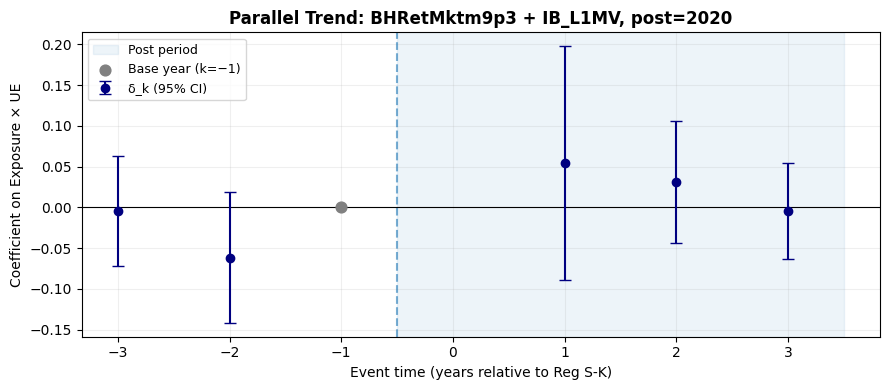
\includegraphics[width=.9\linewidth]{fig_parallel_trend.png}
\caption{Event-Study Coefficients: HCD Intensity $\times$ UE Interaction.
         Dependent variable: market-adjusted buy-and-hold return (m9p3 window).
         UE: income before extraordinary items scaled by lagged market value
         (\texttt{IB\_L1MV}). Mandate year: FY2020. Base year: $k=-1$.
         Coefficients are $\hat{\delta}_k$ on the triple interaction
         $\mathbf{1}[\text{event time}=k] \times HCD_i \times UE_{i,t}$,
         with 95\% confidence intervals. Standard errors clustered by firm.
         Pre-trend F-test: $F=1.32$, $p=0.27$.}
\label{fig:eventstudy}
\end{figure}

%----------------------------------------
% Table 1: Descriptive Statistics
%----------------------------------------
\begin{table}[ht]
\caption{Descriptive Statistics}
\label{tab:descriptives}
\centering
\begin{threeparttable}
\begin{tabular}{lrrrrrrr}
\toprule
Variable & $N$ & Mean & Std.\ Dev. & Min & P25 & Median & Max \\
\midrule
BHRetMktm9p3     & 23,966 &  $-$0.035 & 0.515 & $-$0.866 & $-$0.320 & $-$0.094 & 2.235 \\
BHRetm9p3        & 23,966 &    0.109  & 0.674 & $-$0.874 & $-$0.280 & $-$0.001 & 2.855 \\
IB\_L1MV         & 29,385 & $-$0.117  & 0.495 & $-$3.161 & $-$0.106 &  0.021   & 0.628 \\
c1IB\_L1MV       & 29,358 &    0.025  & 0.435 & $-$1.649 & $-$0.034 &  0.002   & 3.016 \\
HCD (raw)        & 32,448 &    0.011  & 0.007 &  0.000   &  0.007   &  0.010   & 0.074 \\
HCD (std.)       & 32,448 &    0.015  & 0.998 & $-$1.630 & $-$0.597 & $-$0.170 & 9.561 \\
\bottomrule
\end{tabular}
\footnotesize{Notes: Sample is the main estimation sample (post=2020,
$\pm$3-year window, winsorized at 1\%). HCD intensity is the average annual
fraction of human capital words in 10-K filings over FY2015--2019, constructed
from the \citet{demers2024} lexicon. BHRet: raw buy-and-hold return;
BHRetMkt: market-adjusted buy-and-hold return (m9p3 window = April of fiscal
year $t$ through March of $t+1$). IB\_L1MV: income before extraordinary items
scaled by lagged market value. c1IB\_L1MV: year-over-year change in IB\_L1MV.}
\end{threeparttable}
\end{table}

%----------------------------------------
% Table 2: Main Regression Results
%----------------------------------------
\begin{table}[ht]
\caption{Main ERC Regression Results: Effect of HCD Mandate on Earnings Informativeness}
\label{tab:estimates}
\centering
\begin{threeparttable}
\begin{tabular}{lcccc}
\toprule
 & \multicolumn{2}{c}{Market-Adjusted} & \multicolumn{2}{c}{Raw} \\
\cmidrule(lr){2-3}\cmidrule(lr){4-5}
 & BHRetMktm9p3 & BHRetMktm12p & BHRetm9p3 & BHRetm12p \\
 & $\pm$3 yrs   & $\pm$3 yrs   & $\pm$3 yrs & $\pm$3 yrs \\
\midrule
$\beta_1$: $UE$                     &  0.000  &$-$0.036 &$-$0.005 &$-$0.028 \\
$\beta_2$: $Post \times UE$          &$-$0.116***&  0.012 &$-$0.115***&  0.011 \\
$\beta_3$: $HCD \times UE$          &$-$0.044*&$-$0.046**&$-$0.046 &$-$0.048* \\
\midrule
$\beta_4$: $Post \times HCD \times UE$ & 0.098*** & 0.084*** & 0.102** & 0.088** \\
\midrule
$N$                                  & 23,286  & 23,283  & 23,286  & 23,283 \\
\bottomrule
\end{tabular}
\footnotesize{Notes: Dependent variable is the buy-and-hold return over the
m9p3 window (April of fiscal year $t$ through March of $t+1$), either raw
(BHRet) or market-adjusted (BHRetMkt). UE: income before extraordinary items
(\texttt{ib}) scaled by lagged market value (\texttt{IB\_L1MV}). Post: fiscal
year $\geq 2020$. HCD: standardized pre-mandate HCD intensity (FY2015--2019
average, \citet{demers2024} lexicon). All specifications include firm and year
fixed effects. Standard errors clustered by firm in parentheses (omitted for
brevity; see text). ***$p<0.01$; **$p<0.05$; *$p<0.10$.}
\end{threeparttable}
\end{table}

\end{document}
